\documentclass{article}
\usepackage{tikz-feynman}

\begin{document}

\begin{figure}[h]
    \centering
    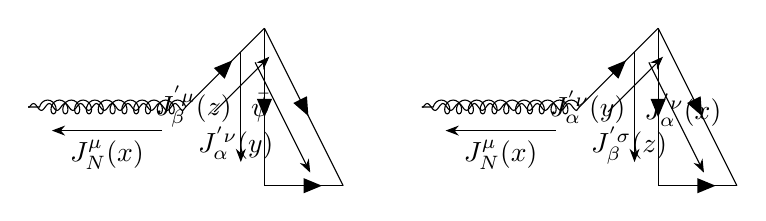
\begin{tikzpicture}
        \begin{feynman}
            \vertex (a) at (-1, 0);
            \vertex (b) at (1, 0);
            \vertex (c) at (2, 1);
            \vertex (d) at (3, -1);
            \vertex (e) at (2, -1);
            \diagram* {
                (a) -- [photon] (b),
                (b) -- [gluon, momentum=\(J^\mu_N(x)\)] (a),
                (b) -- [fermion, momentum'=\(\bar{\psi}\)] (c),
                (c) -- [fermion, momentum'=\(J^{'\nu}_\alpha(y)\)] (d),
                (c) -- [fermion, momentum'=\(J^{'\mu}_\beta(z)\)] (e),
                (d) -- [anti fermion] (e),
            };
        \end{feynman}
        \begin{feynman}[xshift=5cm]
            \vertex (a) at (-1, 0);
            \vertex (b) at (1, 0);
            \vertex (c) at (2, 1);
            \vertex (d) at (3, -1);
            \vertex (e) at (2, -1);
            \diagram* {
                (a) -- [photon] (b),
                (b) -- [gluon, momentum=\(J^\mu_N(x)\)] (a),
                (b) -- [fermion, momentum'=\(J^{'\nu}_\alpha(x)\)] (c),
                (c) -- [fermion, momentum'=\(J^{'\sigma}_\beta(z)\)] (d),
                (c) -- [fermion, momentum'=\(J^{'\nu}_\alpha(y)\)] (e),
                (d) -- [anti fermion] (e),
            };
        \end{feynman}
    \end{tikzpicture}
    \caption{Triangle diagram contributing to the axial anomaly. The axial anomaly leads to non-conservation of the singlet flavour current \( j_0^\mu \), sourced by the dark gluons.}
    \label{fig:triangle_diagram}
\end{figure}

\end{document}